\section{Reading Image Files \& Grayscale Conversion}

Colored images have an interesting, although problematic property; they do not readily lend themselves to matrix manipulation because in order to get color images, seperate values are used to represent each primary color, which are then mixed together for the final color. For example, in Figure~\ref{fig:example}, the block represents very simple a $2 \times 2$ pixel image.

    \begin{figure}[ht]
      \centering
      
\includegraphics[scale=30]{./img/sqr.png}
      \caption{A simple RGB image}
      \label{fig:example}
    \end{figure}

This very simple
image can be
represented as either
a trio of primary
color matrices where
each entry in each
primary        color
matrix coresponds to
the same pixel:

\[
  \underbrace{
    \begin{bmatrix}
      1&0\\
      0&1\\
    \end{bmatrix}
  }_{\text{Red
  Matrix}}
  ,
  \underbrace{
    \begin{bmatrix}
      0&0\\
      1&1\\
    \end{bmatrix}
  }_{\text{Blue
  Matrix}}
  ,
  \underbrace{
    \begin{bmatrix}
      0&1\\
      0&0\\
    \end{bmatrix}
  }_{\text{Green
  Matrix}}
\]

A
single
matrix
may
be
used,
with
each
entry
being
a
submatrix,
wherein
each
element
in
the
submatrix
corresponds
to
a
primary
color.

\[  
  \begin{bmatrix}
    \begin{bmatrix}1\\0\\0\end{bmatrix}
    &
    \begin{bmatrix}0\\1\\0\end{bmatrix}\\[2em]
    \begin{bmatrix}0\\0\\1\end{bmatrix}
    &
    \begin{bmatrix}1\\0\\1\end{bmatrix}
  \end{bmatrix}
\]

Using
one
of
the
given
images,
the
splitting
of
color
channels
gives
the
following
set
of
images
shown
in
Figure~\ref{3color}.

\begin{figure}[ht]
  \centering
  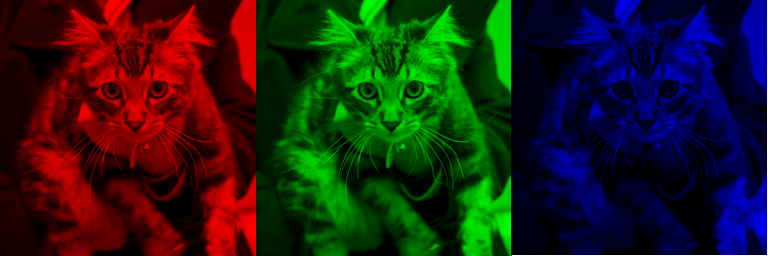
\includegraphics[scale=0.4]{./img/photo2-exploded.png}
  \caption{A
    given
    image
    split
    into
    its
    three
    primary
    color
  channels}
  \label{3color}
\end{figure}

While
it
is
possible
to
manipulate
color
images,
it
would
be
far
simpler
to
manipulate
\emph{grayscale}
images,
where
only
the
final
intensity
is
concerned.
To
do
this,
each
color
is
considered
independently
for
its
intensity
alone
as
shown
in
Figure~\ref{3gray},
where
it
may
be
scaled,
and
then
added
together
to
produce
a
final
black-and-white
image,
which
is
a
matrix
where
each
entry
is
a
single
value.
Note
how
the
third
panel
representing
the
blue
color
channel
is
darker
--
this
implies
that
blue
is
a
less
intense
color
in
the
image.

\begin{figure}[ht]
  \centering
  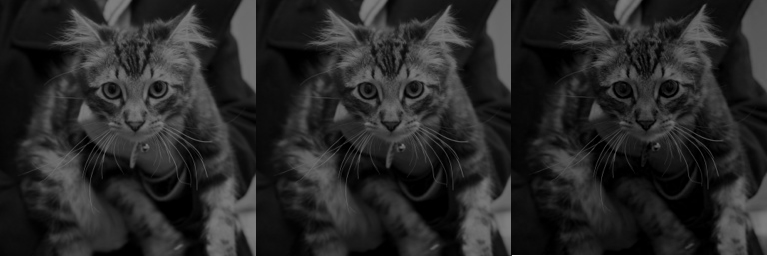
\includegraphics[scale=0.4]{./img/photo2-explodedg.png}
  \caption{A
    given
    image
    split
    into
    its
    three
    primary
    color
    channels,
    but
    only
    intensity
    of
    each
    color
    is
  shown.}
  \label{3gray}
\end{figure}

Since each primary color is freely editable, it is simple to scale the
intensity of each before mixing; in our report, we    used 30\% of the red
channel, 59\% of the green channel and 11\% of the blue channel. The final
outputs for both given       images can be seen in
Figure~\ref{fig:gray_images}. Note how the final output is lighter than any of
the individual color    channels.

\begin{figure}[ht]
  \centering
  \begin{subfigure}{\textwidth}
    \centering
    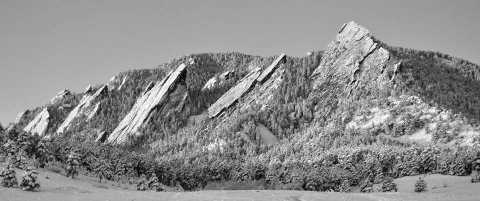
\includegraphics[scale=0.4]{./img/gray1.png}
    \caption{Photo 1 -
    Grayscale}
    \label{fig:p1g}
  \end{subfigure}
  \begin{subfigure}{\textwidth}
    \centering
    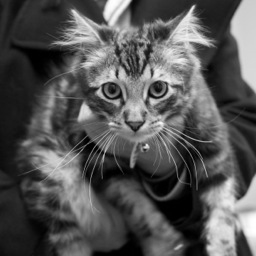
\includegraphics[scale=0.4]{./img/gray2.png}
    \caption{Photo
      2
      -
    Grayscale}
    \label{fig:p2g}
  \end{subfigure}
  \caption{Grayscale
  Images}
  \label{fig:gray_images}
\end{figure}

